\begin{figure*}[t]
    \centering
    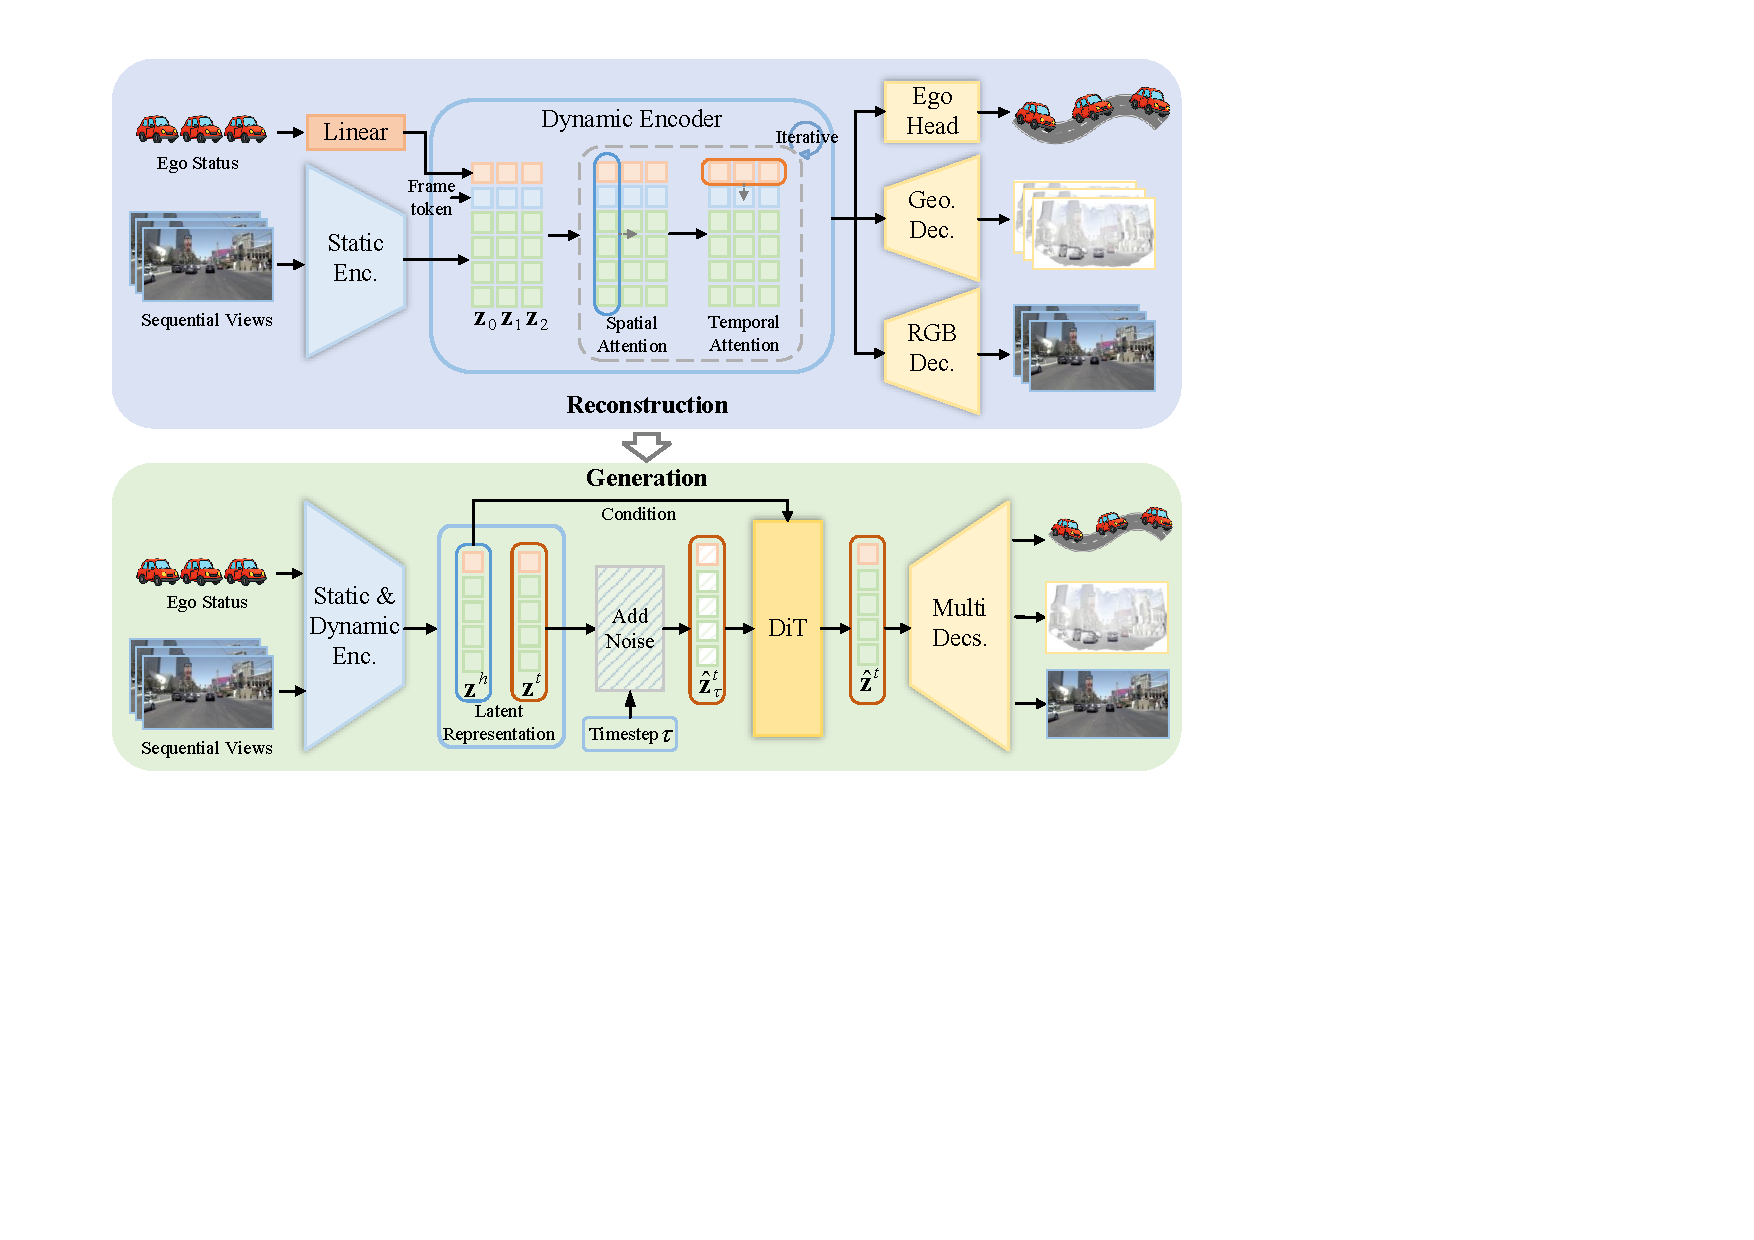
\includegraphics[width=0.9\textwidth]{imgs/framework.pdf}
    \caption{\textbf{The overall framework of our UniDWM.} UniDWM is composed of the Reconstruction and Generation stages. Given a sequence of visual observations as input, UniDWM projects them to a unified feature space using static and dynamic encoders. Then, reconstruction and generation decoders can be used to reconstruct the observed scene and generate dynamic evolution, respectively. }
    \label{fig_framework}
\end{figure*}

\section{Method}

\subsection{Preliminary}

Variational Autoencoder (VAE)~\cite{kingma2014auto} is a probabilistic generative framework that introduces latent variables
$z \in \mathcal{Z}$ to explain observations $\mathbf{x} \in \mathcal{X}$.
The model assumes a simple prior distribution $p(\mathbf{z})$ over the latent space, commonly chosen as a Gaussian distribution,
and defines a conditional data distribution $p_\theta(\mathbf{x} | \mathbf{z})$ parameterized by a neural network.
Given the data-generating distribution $p_{\mathcal{D}}(\mathbf{x})$, approximated by a finite training set,
learning is naturally formulated as maximizing the expected marginal log-likelihood:
\begin{equation}
\mathbb{E}_{p_{\mathcal{D}}(\mathbf{x})} \big[ \log p_\theta(\mathbf{x}) \big]
=
\mathbb{E}_{p_{\mathcal{D}}(\mathbf{x})} \Big[ \log \mathbb{E}_{p(\mathbf{z})} \big[ p_\theta(\mathbf{x} \mid \mathbf{z}) \big] \Big].
\label{Eq:vae_likelihood}
\end{equation}
Directly optimizing this objective is generally infeasible due to the intractable integration over latent variables.
To overcome this difficulty, VAE introduces a variational posterior $q_\phi(\mathbf{z} | \mathbf{x})$
and maximizes a tractable lower bound of the log-likelihood, given by:
\begin{equation}
\mathcal{L}_{\text{VAE}} =
\mathbb{E}_{q_\phi(\mathbf{z} \mid \mathbf{x})} \big[ \log p_\theta(\mathbf{x} \mid \mathbf{z}) \big]
-
\mathrm{KL}\!\left(q_\phi(\mathbf{z} \mid \mathbf{x}) \,\|\, p(\mathbf{z})\right),
\label{Eq:vae}
\end{equation}
which satisfies $\mathcal{L}_{\text{VAE}} \le \log p_\theta(\mathbf{x})$.

While effective in practice, the standard VAE objective implicitly limits the mutual information between observations and latent variables,
often resulting in weakly informative representations.
InfoVAE~\cite{zhao2017infovae} alleviates this issue by decoupling information preservation from prior regularization.
The resulting objective is formulated as: 
\begin{equation}
\begin{aligned}
\mathcal{L}_{\text{InfoVAE}} \equiv\;&
\mathbb{E}_{p_{\mathcal{D}}(\mathbf{x})}
\mathbb{E}_{q_\phi(\mathbf{z} \mid \mathbf{x})}
\big[ \log p_\theta(\mathbf{x} \mid \mathbf{z}) \big] \\
&- (1 - \alpha)\,
\mathbb{E}_{p_{\mathcal{D}}(\mathbf{x})}
\mathrm{KL}\!\left(q_\phi(\mathbf{z} \mid \mathbf{x}) \,\|\, p(\mathbf{z})\right) \\
&- (\alpha + \lambda - 1)\,
\mathrm{D}\!\left(q_\phi(\mathbf{z}) \,\|\, p(\mathbf{z})\right),
\end{aligned}
\label{Eq:infovae}
\end{equation}
where $q_\phi(z) = \mathbb{E}_{p_{\mathcal{D}}(x)} q_\phi(z | x)$ denotes the aggregated posterior.
Here, $D(\cdot\|\cdot)$ represents a divergence measure such as KL divergence or maximum mean discrepancy, and the hyperparameters $\alpha$ and $\lambda$ balance reconstruction fidelity, prior matching, and information preservation.

\subsection{Unified Driving World Model}
We consider a driving dataset $\mathcal{D} = \{ \mathbf{x}_i \in \mathcal{X}\}_{i=1}^{N}$ of $N$ i.i.d. scenes, each of which is a set of $M$ observations $\mathbf{x}_i = \{\boldsymbol{x}_i^{(j)}\}_{j=1}^{M}$ from different perspectives. We consider a frame with a single modality as an observation perspective. If a scene in the dataset is composed of $l$ frames and $m$ modalities (e.g., points, images, ego poses, etc.), then $M$ is equal to $l \times m$. Given some local observations $\mathbf{x}^{local} \in \mathbf{x}$ of a scene, the objective of UniDWM is reconstruct the global observations $\mathbf{x}$. The ELBO of UniDWM can be written as:
\begin{equation}
\begin{aligned}
\mathcal{L}_{\text{UniDWM0}} \equiv\;&
 {\textstyle \sum_{j=1}^{M}} \mathbb{E}_{p_{\mathcal{D}}(\mathbf{x})}
\mathbb{E}_{q_\phi(\mathbf{z} \mid \mathbf{x}^{local})}
\big[ \log p_\theta(\boldsymbol{x}^{(j)} \mid \mathbf{z}) \big] \\
&- 
\mathbb{E}_{p_{\mathcal{D}}(\mathbf{x})}
\mathrm{KL}\!\left(q_\phi(\mathbf{z} \mid \mathbf{x}^{local}) \,\|\, p(\mathbf{z})\right), \\
\end{aligned}
\label{Eq:unidwm0}
\end{equation}
where $z \in \mathcal{Z}$ denotes the latent variable, $p_{\theta}(\boldsymbol{x}^{(j)}|\mathbf{z})$ represents single-modality conditional distribution, and $q_{\phi}(z | \mathbf{x}^{local})$ is the approxiation posterior given local observations. A proof can be found in Appendix~\ref{vae_unidwm}. However, the VAE-style ELBO may fail to learn meaningful latent representation, especially when the data space $\mathcal{X}$ is complex and high-dimensional. Therefore, we conclude another ELBO objective inspired by InfoVAE:
\begin{equation}
\begin{aligned}
\mathcal{L}_{\text{UniDWM}} =&
 {\textstyle \sum_{j=1}^{M}} \mathbb{E}_{p_{\mathcal{D}}(\mathbf{x})}
\mathbb{E}_{q_\phi(\mathbf{z} \mid \mathbf{x}^{local})}
\big[ \log p_\theta(\boldsymbol{x}^{(j)} \mid \mathbf{z}) \big] \\
% &- (1 - \alpha)
% \mathbb{E}_{p_{\mathcal{D}}(\mathbf{x})}
% \mathrm{KL}\!\left(q_\phi(\mathbf{z} \mid \mathbf{x}^{local}) \,\|\, p(\mathbf{z})\right) \\
&- \lambda D(q_{\phi}(\mathbf{z})\,\|\,p(\mathbf{z})), \\ 
\end{aligned}
\label{Eq:unidwm}
\end{equation}
which is similar to Eq.~\ref{Eq:infovae}, but with multi-observation reconstruction and setting $a=1$. A proof can be seen in Appendix~\ref{infovae_unidwm}. In practice, we employ the SIGReg \cite{balestriero2025lejepa} as the regulation term $D(\cdot\|\cdot)$. SIGReg applies the Epps-Pulley test to measure the distribution discrepancy, which satisfies the requirement of InfoVAE ($D(q_\phi(z) \|\ p(z)) = 0$ iff $q_\phi(z) = p(z)$). The log-likelihood terms are implemented as the negative reconstruction and generation losses $\mathcal{L}_{recon}$ and $\mathcal{L}_{gen}$, which will be detailed in Sec.~\ref{recon} and Sec.~\ref{gen}.

\subsection{Framework of UniDWM}
% The framework of UniDWM is shown in Figure~\ref{fig_framework}. We encode the driving scene as a unified world representation where ego motion, geometry, and appearance are encoded in the shared latent space. UniDWM employs a spatiotemporal encoder–decoder architecture. The encoder compresses sensory inputs into a compact latent feature field, while the decoder family reconstructs different aspects of the physical scene from it. To achieve such multifaceted representation learning, UniDWM first adopts \textbf{\textit{Joint Reconstruction}} (Sec.~\ref{recon}), which learns a global world representation by reconstructing geometry, appearance, and ego-motion from local observations. Then the pretrained model is fine-tuned in the \textbf{\textit{Collaborative Generation}} (Sec.~\ref{gen}) stage to encode dynamic clues in the latent world representation. Together, these components enable UniDWM to not only act as a self-supervised foundation model to learn a global world representation, but also to support extensive applications, including reasoning about geometric and visual structures (perception), the dynamics of surrounding agents (prediction), and ego-motion evolution (planning) within a single unified model.
The overall framework of UniDWM is illustrated in Figure~\ref{fig_framework}. UniDWM adopts a spatiotemporal encoder–decoder architecture: the encoder compresses visual inputs into a compact latent feature field, while a family of decoders reconstructs different physical aspects of the driving scene from this representation. To enable such comprehensive representation learning, UniDWM first introduces \textbf{\textit{Joint Reconstruction}} (Sec.~\ref{recon}), which guides the encoder be aware of spatial structure by jointly reconstructing geometry, appearance, and ego motion from local observations. Subsequently, the pretrained model is fine-tuned in the \textbf{\textit{Collaborative Generation}} stage (Sec.~\ref{gen}) to further encode dynamic cues into the latent world representation. Together, these components allow UniDWM to function not only as a self-supervised foundation model for world modeling but also as a unified framework supporting a wide range of downstream tasks, including reasoning about geometric and visual structures (perception), modeling the dynamics of surrounding agents (prediction), and capturing ego-motion evolution (planning).

% \noindent\textbf{Multimodal latent world representation.}
% At the core of UniDWM lies a unified latent world representation that captures both the spatial and temporal structure of the driving environment. Rather than handling geometry, appearance, and ego-motion as independent components, we represent the driving scene as a shared latent state $\mathbf{z}$ that serves as the common generative source for all physical modalities. This latent formulation provides a modality-agnostic abstraction, allowing the model to jointly reason about 3D geometry, visual appearance, and dynamic motion in a coherent embedding space.

\subsection{Joint Reconstruction}
\label{recon}
To learn a physically grounded latent world representation, we construct the world representation through a joint 4D scene reconstruction pathway that reconstructs 3D geometry, visual appearance, and ego motion over time. Specifically, we adopt a variational autoencoding architecture, where a shared spatiotemporal encoder $q_\phi$ compresses a sequence of visual observations $I_{1:n}$ and ego status $s_{1:n}$ into a unified latent embedding $\mathbf{z}$:
\begin{equation}
    \mathbf{z} \sim q_\phi(\mathbf{z}\mid I_{1:n}, s_{1:n}),
\end{equation}
where $\mathbf{z}$ is designed to be \textit{modality-agnostic} and \textit{time-continuous}, enabling it to jointly encode 3D structural priors, temporal motion cues, and visual appearance information within a shared latent space. The shared spatiotemporal encoder consists of two complementary components: a static encoder and a dynamic encoder. 

\noindent\textbf{Static Encoder.} To reduce training overhead and stabilize the representation learning, we reuse a pretrained encoder \cite{dcae, dinov3} as the static encoder, which is responsible for capturing view-consistent features from individual frames. The parameters of this static encoder are frozen during training to preserve general low-level representations. The ego status is encoded by an MLP. A deep-spatial-compressed latent state $\textbf{z}\in \mathbb{R}^{n\times (l+1) \times c}$ is obtained:
\begin{equation}
    \begin{aligned}
     \textbf{z}_{rgb} = \text{Encoder}(I_{1:n}) \in \mathbb{R}^{n\times l \times c}, \\
     \textbf{z}_{ego} = \text{MLP}(s_{1:n}) \in \mathbb{R}^{n\times 1 \times c}, \\
     \textbf{z} = \text{Concatenate}([\textbf{z}_{rgb},\textbf{z}_{ego}]),
    \end{aligned}
    \label{Eq:s_encoder}
\end{equation}
\noindent where $c$ is the channel number, $l$ is the length of tokens of each frame.

\begin{figure}[t]
    \centering
    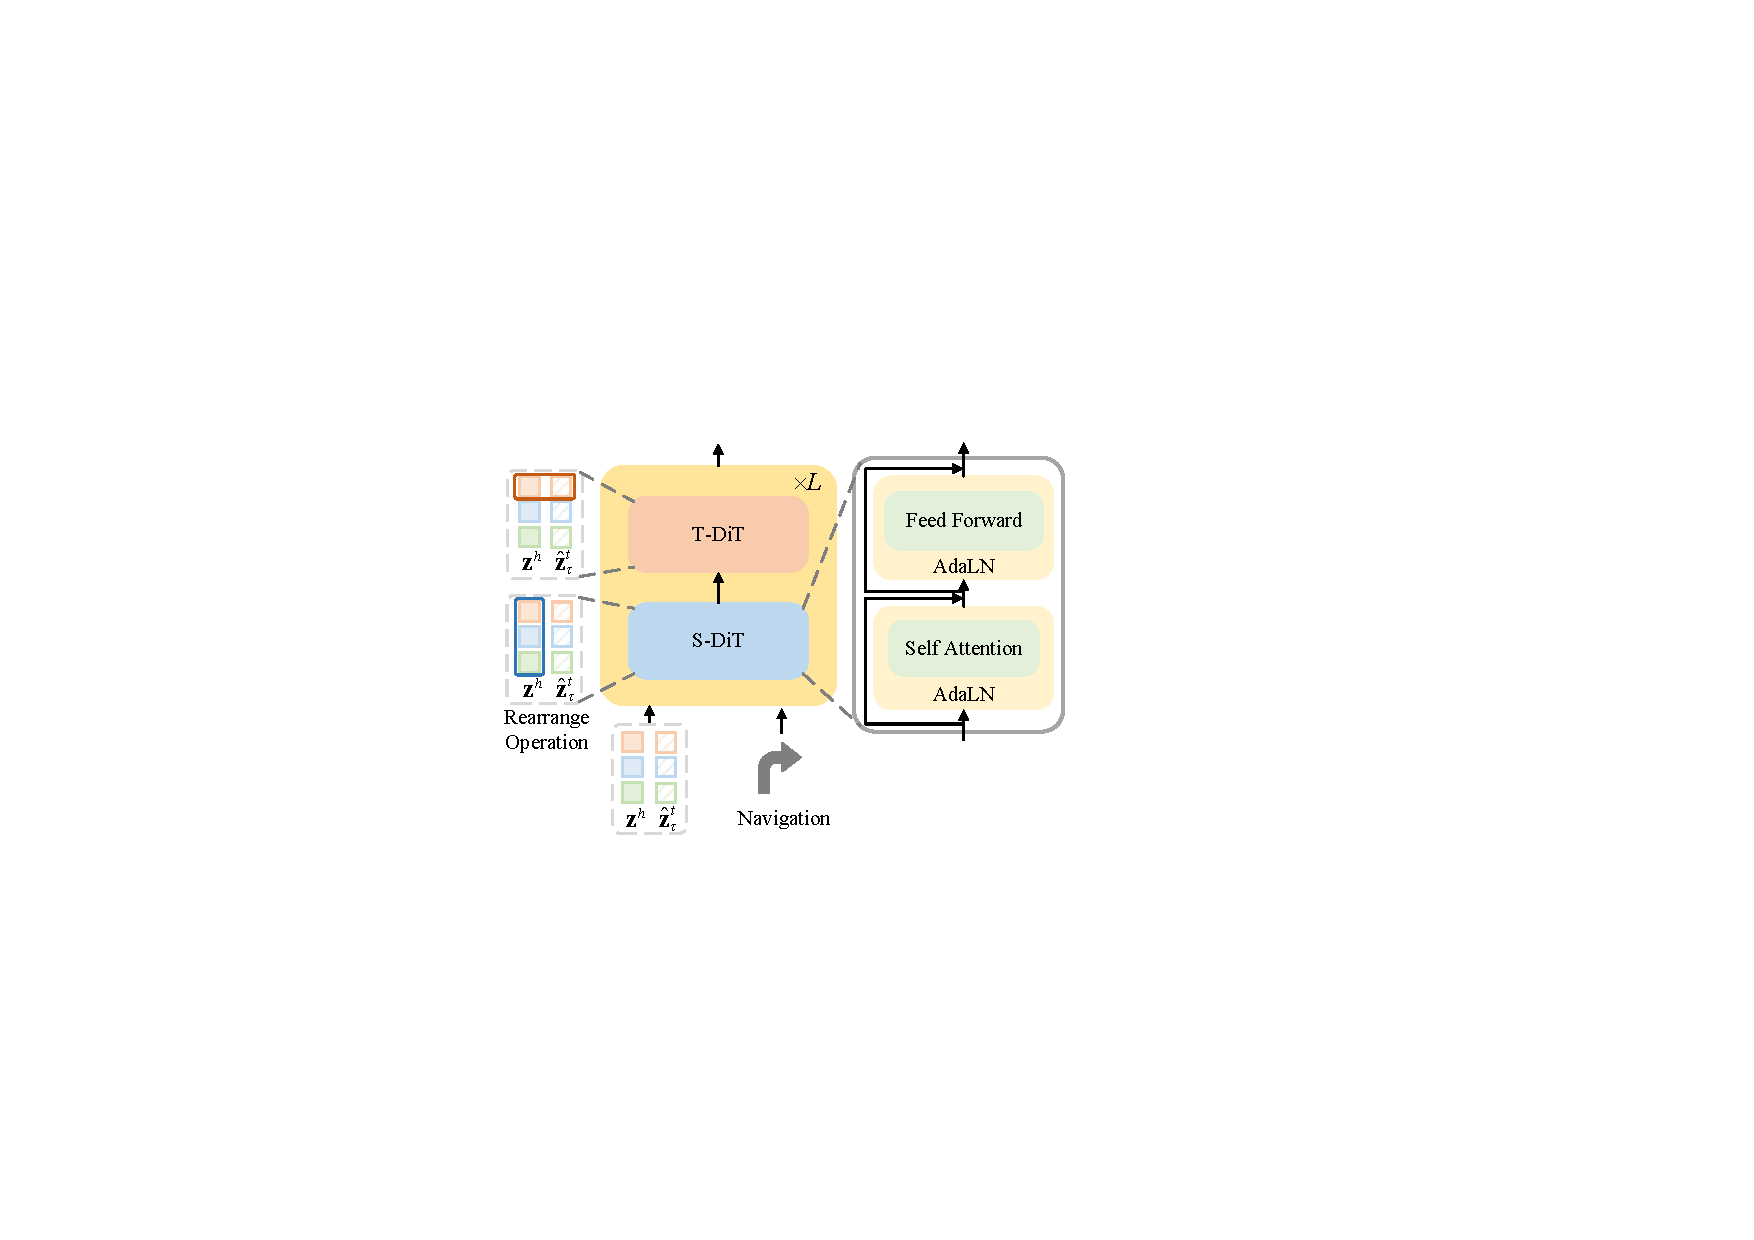
\includegraphics[width=1.0\columnwidth]{imgs/dit_framework.pdf}
    \caption{\textbf{Architecture of the DiT block}, consisting of an alternating sequence of spatial DiT (S-DiT) and temporal DiT (T-DiT) modules. }
    \label{fig_causal}
\end{figure}

% \begin{figure}[t]
%     \centering
%     
\includegraphics[width=0.8\columnwidth]{causal_mask.pdf}
%     \caption{\textbf{Casual mask in temporal attention.} `rand' represents that the value of the grid is generated by calling the rand function. Finally, the grid value in the causal mask matrix is set to inf' if it is smaller than a hyper-parameter `p', else it is set to 1.}
%     \label{fig_causal}
% \end{figure}

\noindent\textbf{Dynamic Encoder.} The dynamic encoder is designed to model scene evolution and ego dynamics over time. Inspired by recent advances in spatiotemporal and geometry modeling~\cite{hu2024drivingworld, epona, vggt}, we construct the dynamic encoder by alternately stacking spatial and temporal attention layers. The architecture of the dynamic encoder is shown in Figure~\ref{fig_framework}. The spatial attention aggregates geometric and contextual features within each frame, while the temporal attention captures inter-frame motion and continuity in the latent domain. This alternating structure enables effective cross-frame interaction and smooth temporal reasoning, ensuring that the resulting latent representation $\mathbf{z}$ reflects a consistent 4D understanding of the driving scene. Specifically, a stack of $L$ layers of spatial-temporal transformers is employed to capture the structure information of the driving scene progressively:
\begin{equation}
    \begin{aligned}
     \textbf{z} & \gets  \text{SpatialAttn}(\textbf{z}), \\
     \textbf{z} &\gets  \text{TemporalAttn}(\textbf{z},
     \mathcal{M}),
    \end{aligned}
    \label{Eq:d_encoder}
\end{equation}
\noindent where $\mathcal{M}\in \mathbb{R}^{n \times n}$ is a causal mask that is used to keep information flowing unidirectionally over time. 

\noindent\textbf{Decoupled Decoders.}
Given the shared latent world representation $\mathbf{z}$, the objective is to reconstruct geometry, visual appearance, and ego motion, respectively. Since these modalities reside in distinct feature domains, we design decoupled decoders that project $\textbf{z}$ into their respective feature spaces:
\begin{equation}
\begin{aligned}
    \{\hat{\textbf{D}}, \hat{\textbf{P}},\Sigma_{d},\Sigma_{p}  \} =\mathcal{D}^{\text{geo}}(\textbf{z}), \\
    \hat{\textbf{C}} = \mathcal{D}^{\text{rgb}}(\textbf{z}), \hat{\textbf{e}}=\mathcal{D}^{\text{ego}}(\textbf{z}),
\end{aligned}
\end{equation}
where $\{\hat{\textbf{D}} \in \mathbb{R}^{n\times H \times W \times 3},\hat{\textbf{P}} \in \mathbb{R}^{n\times H \times W \times 1}\}$ denote the reconstructed geometry attributes (points and depths). $\{\Sigma_d, \Sigma_p\}$ represent the aleatoric uncertainty \cite{kendall2016modelling, novotny2018capturing} of depth and point predictions. $\hat{\textbf{C}} \in \mathbb{R}^{n \times H \times W \times 3}$, and $\hat{\textbf{e}} \in \mathbb{R}^{n \times 3}$ denote the visual appearance (RGB colors) and ego poses (ego center and heading), respectively. 

For geometry and appearance reconstruction, we build decoders following prior methods \cite{dcae, rae}. In practice, $\mathcal{D}^{\text{rgb}}$ are initialized from the pretrained decoder weights \cite{dcae, rae} and frozen during training. For the ego-motion decoder, following VGGT~\cite{vggt}, we employ a lightweight transformer-based decoder composed of four self-attention layers followed by a linear projection head.

\noindent\textbf{Reconstruction Loss. }
We employ three kinds of loss to build the reconstruction loss:
\begin{equation}
   \mathcal{L}_{recon} = \mathcal{L}_{ego} + \mathcal{L}_{geo} + \mathcal{L}_{vis},
\end{equation}
\noindent where $\mathcal{L}_{ego}$, $\mathcal{L}_{geo}$, and $\mathcal{L}_{vis}$ are ego motion, geometry, and visual appearance losses, respectively. $\mathcal{L}_{ego}$ is calculated by comparing the L2 distance between the predicted ego poses $\hat{\textbf{e}}$ and ground-truth ego poses \textbf{e}: $\mathcal{L}_{ego} = \frac{1}{n}||\hat{\textbf{e}} - \textbf{e}||_2$. Following prior work \cite{vggt}, $\mathcal{L}_{geo}$ is calculated as follows:
\begin{equation}
\begin{aligned}
    \mathcal{L}_{geo} =& \mathcal{L}_{\text {depth }}  + \mathcal{L}_{\text {point }},\\
    \mathcal{L}_{\text {depth }} =&\frac{1}{n} \| \Sigma_{d} \left(\hat{\textbf{D}}-\textbf{D}\right)\|+ \\ &\frac{1}{n}\|\Sigma_{d} \odot\left(\nabla \hat{\textbf{D}}-\nabla \textbf{D}\right) \|-a \log \Sigma_{d},\\
    \mathcal{L}_{\text {points}} =&\frac{1}{n} \| \Sigma_{p} \left(\hat{\textbf{P}}-\textbf{P}\right)\|+ \\ &\frac{1}{n}\|\Sigma_{p} \odot\left(\nabla \hat{\textbf{P}}-\nabla \textbf{P}\right) \|- a \log \Sigma_{p},\\
\end{aligned}
\end{equation}
\noindent where $\odot$ denotes the channel-broadcast element-wise product, $\Sigma_{d}$ and $\Sigma_{p}$ represent the depth and point uncertainty map, respectively. $\mathcal{L}_{rgb}$ is calculated as follows:
\begin{equation}
\begin{aligned}
    \mathcal{L}_{vis} =& \|\hat{\textbf{C}} - \textbf{C}\|  + \omega_{l}\text{LPIPS}(\hat{\textbf{C}}, \textbf{C}) + \omega_{g} \mathcal{L}_{GAN},\\
\end{aligned}
\end{equation}
\noindent where $\text{LPIPS}(\cdot)$ denotes the LPIPS \cite{lpips} function, $\mathcal{L}_{GAN}$ is GAN loss as in \cite{gan_loss, rae}. $\omega_l$ and $\omega_g$ are weights for LPIPS and GAN loss and are set to $1.0$ and $0.75$ in practice following \cite{rae}.

\subsection{Collaborative Generation}
\label{gen}

While joint 4D scene reconstruction enables the model to learn a physically grounded latent representation of the observed scenes, autonomous driving requires not only understanding but also \emph{forecasting} future dynamics. To achieve such a goal, we introduce a \textit{collaborative generation} framework that models future world evolution as a conditional generative process in the latent space. By jointly sampling future 4D scene latents conditioned on historical context, the model achieves coherent forecasting across different tasks, enabling unified imagination of both future scenes and agent behaviors. Note that generation modules can also be seen as decoders for future observations that enable UniDWM with dynamic imagination capability. 

Specifically, given the latent world representation $\mathbf{z}^{h}\in \mathbb{R}^{n^h \times (l + 1) \times c}$ encoded from historical visual observations and ego poses, our diffusion-based generator aims to synthesize the future latent world representation $\mathbf{z}^{t} \in \mathbb{R}^{n^t \times (l + 1) \times c}$ for 4D generation and planning. Following prior works \cite{kong2024hunyuanvideo, epona}, the generation process is implemented using a conditional DiT framework; the detailed architecture is shown in Figure~\ref{fig_causal}. The DiT framework is also composed of spatial and temporal attention layers similar to the dynamic encoder, but with AdaLN layers to adapt to the timestep and guidance information. 


\begin{table*}[t]
\centering
% \resizebox{\linewidth}{!}{
\caption{\textbf{Performance on the NAVSIM \textit{navtest} split.} `*' denotes the results obtained by ourselves. `Percep. Label' denotes the required perception labels for a method. `C', `L', and `E' represent camera, LiDAR, and ego status inputs, respectively. The best results of methods with and without perception labels are highlighted in \textbf{bold}, respectively. }
\begin{tabular}{lccccccc}
\toprule
\textbf{Method} & \textbf{Input} & \textbf{Percep. Label} & \textbf{NC} $\uparrow$ & \textbf{DAC} $\uparrow$ & \textbf{EP} $\uparrow$ & \textbf{TTC} $\uparrow$ & \textbf{PDMS} $\uparrow$ \\
\midrule
UniAD \cite{hu2023planning} & C & BBox, Map, Occ & 97.8 & 91.9 & 78.8 & 92.9 & 83.4 \\
LTF \cite{transfuser} & C & BBox, Map & 97.4 & 92.8 & 79.0 & 92.4 & 83.8 \\
TransFuser \cite{transfuser} & C \& L & BBox, Map & 97.7 & 92.8 & 79.2 & 93.0 & 84.0 \\
Hydra-MDP \cite{li2024hydra} & C \& L & BBox, Map & 98.3 & 96.0 & 78.7 & 94.6 & 86.5 \\
DiffusionDrive \cite{liao2025diffusiondrive} & C \& L & BBox, Map & 98.2 & 96.2 & 82.2 & 94.7 & 88.1 \\
GoalFlow \cite{xing2025goalflow} & C \& L & BBox, Map & 98.4 & \textbf{98.3} & 85.0 & 94.6 & 90.3 \\
GaussianFusion \cite{liu2025gaussianfusion} & C \& L & BBox, Map & \textbf{98.7} & 98.1 & \textbf{88.2} & \textbf{95.7} & \textbf{92.0} \\
\hline
Ego-MLP & E & None & 93.0 & 77.3 & 62.8 & 83.6 & 65.6 \\
LAW \cite{law} & C & None & 97.2 & 93.3 & 78.8 & 91.9 & 83.8 \\
World4Drive \cite{zheng2025world4drive} & C & None & 97.4 & 94.3 & 79.9 & 92.8 & 85.1 \\
DINOv3 (B)$^*$ \cite{dinov3} & C & None & 97.8 & 94.4 & 80.2 & 93.0 & 85.4 \\
Epona \cite{epona} & C & None & 97.9 & 95.1 & 80.4 & 93.8 & 86.2 \\
\rowcolor{cyan!20}
UniDWM (DCAE) & C & None & 97.4 & 93.2 & 80.1 & 93.3 & 84.9 \\
\rowcolor{cyan!20}
UniDWM (DINOv3-B) & C & None & \textbf{98.3} & \textbf{97.9} & \textbf{86.0} & \textbf{95.1} & \textbf{90.6} \\
\bottomrule
\end{tabular}
\label{tab:navsim_pdms}
\end{table*}


% \begin{table*}[t]
% \centering
% % \resizebox{\linewidth}{!}{
% \begin{tabular}{lccccccc|c}
% \toprule
% \textbf{Method} & \textbf{NC} $\uparrow$ & \textbf{DAC} $\uparrow$ & \textbf{EP} $\uparrow$ & \textbf{TTC} $\uparrow$ & \textbf{DDC} $\uparrow$ & \textbf{LK} $\uparrow$ & \textbf{EC} $\uparrow$ & \textbf{EPDMS} $\uparrow$ \\
% \midrule
% % PDM-closed \cite{pdm-closed} & 94.6 & 99.8 & 89.9 & 86.9 & 98.7 & 66.7 & 98.0 & 82.8 \\

% TransFuser$^{*}$~\cite{transfuser} & 97.7 & 92.8 & 79.2 & 92.8 & 98.3 & 67.6 & 95.3 & 77.8 \\
% VADv2$^{*}$~\cite{vadv2} & 97.3 & 91.7 & 77.6 & 92.7 & 98.2 & 66.0 & 97.4 & 76.6 \\
% Hydra-MDP$^{*}$~\cite{li2024hydra} & 97.5 & 96.3 & 80.1 & 93.0 & 98.3 & 65.5 & 97.4 & 79.8 \\
% Hydra-MDP++$^{*}$~\cite{li2025hydra} & 97.9 & 96.5 & 79.2 & 93.4 & 98.9 & 67.2 & 97.7 & 80.6 \\
% ARTEMIS \cite{feng2025artemis} & \textbf{98.3} & 95.1 & 81.5 & 97.4 & 98.6 & 96.5 & 98.3 & 83.1 \\
% DiffusionDrive \cite{diffusiondrive} & 98.2 & 96.2 & \textbf{87.6} & 97.3 & 98.6 & 97.0 & \textbf{98.4} & 84.0 \\
% \rowcolor{cyan!20}
% GaussianFusion (Ours) & \textbf{98.3} & \textbf{97.3}& 87.5 & \textbf{97.4} & \textbf{99.0} & \textbf{97.4} & 98.3 & \textbf{85.0} \\
% \bottomrule
% \end{tabular}
% \caption{\textbf{Performance on the NAVSIM \textit{navtest} split with extended metrics.} `*' represents that the results are sourced from Hydra-MDP++~\cite{li2025hydra}. The best results are highlighted in bold. }
% \label{tab:navsim}
% \end{table*}

In practice, we inject navigation embedding $\mathbf{g}_{\text{nav}}$ as conditional guidance to the DiT blocks. This enables the generator to jointly imagine plausible future latent state $\hat{\mathbf{z}}^{t}$ that are semantically aligned with navigation intent. The conditional generative dynamics are formulated as:
\begin{equation}
    \hat{\mathbf{z}}^{t}_{\tau-1} = 
    \hat{\mathbf{z}}^{t}_{\tau} + \Delta \tau \cdot v_{\Theta}\left(\hat{\mathbf{z}}^{t}_{\tau}, \tau, [\mathbf{z}^{h}, \mathbf{g}_{\text{nav}}]\right),
    \label{eq:stage1}
\end{equation}
where $\hat{\mathbf{z}}^{t}_{\tau}$ denotes the noisy future latent at diffusion timestep $\tau$, $\mathbf{z}^{h}$ represents the historical latent context, and $v_{\Theta}$ is the DiT-based velocity field. The loss for the generation follows the standard velocity prediction objective:
\begin{equation}
    \mathcal{L}_{\text{gen}} = 
    \mathbb{E}_{\mathbf{z}^{t}, \epsilon, \tau}
    \left\|v_{\Theta}\left(\hat{\mathbf{z}}^{t}_{\tau}, \tau, [\mathbf{z}^{h}, \mathbf{g}_{\text{nav}}]\right)
    - (\mathbf{z}^{t} - \epsilon)\right\|^{2},
    \label{eq:loss1}
\end{equation}
where $\mathbf{z}^{t}$ denotes the ground-truth future latent representation, and $\epsilon \sim \mathcal{N}(0, I)$.